\documentclass[11pt]{beamer}
\usepackage[utf8]{inputenc}
\usepackage[T1]{fontenc}
\usepackage{lmodern}
\usepackage[french]{babel}
\usetheme{Antibes}
\usepackage{subfig}
\usepackage{algorithm}
\usepackage{algorithmic}
%%% Packages additionnels
\usepackage{verbatim}
\usepackage{bbm}
\usepackage{stmaryrd}
\usepackage[numbered,framed]{matlab-prettifier}
\usepackage{listings}

\renewcommand{\algorithmicrequire}{\textbf{Entrée(s) :}}
\renewcommand{\algorithmicreturn}{\textbf{retourner}}
\renewcommand{\algorithmicensure}{\textbf{Initialisation ;}}
\renewcommand{\algorithmicwhile}{\textbf{Tant que}}
\renewcommand{\algorithmicdo}{\textbf{Initialisation}}
\renewcommand{\algorithmicendwhile}{\textbf{fin du Tant que ;}}
\renewcommand{\algorithmicend}{\textbf{fin}}
\renewcommand{\algorithmicif}{\textbf{si}}
\renewcommand{\algorithmicendif}{\textbf{fin du si}}
\renewcommand{\algorithmicelse}{\textbf{sinon}}
\renewcommand{\algorithmicelsif}{\textbf{fin du sinon}}
\renewcommand{\algorithmicthen}{\textbf{alors}}
\renewcommand{\algorithmicthen}{\textbf{Étape E}}
\renewcommand{\algorithmicthen}{\textbf{Étape M}}
\renewcommand{\algorithmicfor}{\textbf{pour}}
\renewcommand{\algorithmicforall}{\textbf{pour tout}}
\renewcommand{\algorithmicto}{\textbf{à}}
\renewcommand{\algorithmicendfor}{\textbf{fin du pour}}
\renewcommand{\algorithmicdo}{\textbf{faire}}
\renewcommand{\algorithmicloop}{\textbf{boucler}}
\renewcommand{\algorithmicendloop}{\textbf{fin de la boucle}}
\renewcommand{\algorithmicrepeat}{\textbf{répéter}}
\renewcommand{\algorithmicuntil}{\textbf{jusqu’à}}

\setbeamertemplate{blocks}[rounded][shadow=true]
\makeatother
\setbeamertemplate{footline}
{
	\leavevmode%
	\hbox{%
		\begin{beamercolorbox}[wd=.33\paperwidth,ht=2.25ex,dp=1ex,center]{author in head/foot}%
			\usebeamerfont{author in head/foot}\insertshortauthor
		\end{beamercolorbox}%
		\begin{beamercolorbox}[wd=.33\paperwidth,ht=2.25ex,dp=1ex,center]{title in head/foot}%
			\usebeamerfont{title in head/foot}\insertshorttitle
		\end{beamercolorbox}%
		\begin{beamercolorbox}[wd=.33\paperwidth,ht=2.25ex,dp=1ex,center]{date in head/foot}%
			\usebeamerfont{date in head/foot}\insertshortdate\hspace*{3em}
			\insertframenumber{} / \inserttotalframenumber\hspace*{1ex}
	\end{beamercolorbox}}%
	\vskip0pt%
}
\makeatletter
\setbeamertemplate{itemize item}[ball]
\setbeamertemplate{itemize subitem}[triangle]
\setbeamertemplate{itemize subsubitem}[circle]



\AtBeginSection[]{\begin{frame} \tableofcontents[currentsection] \end{frame}}


\begin{document}
	\author{SENE, CÔME, PRALON}
	\title[Projet UE HAX907X]{Détection de structures communautaires dans des réseaux}
	\subtitle{}
	\logo{
		\begin{minipage}[c]{1.15\linewidth}
			
\includegraphics[height=0.6cm]{images/logo.png} \hspace{0.65truecm}\hfill 
			
\includegraphics[height=0.6cm]{images/imag_logo.png}
			\hspace{0.65truecm}\hfill 
			
\includegraphics[height=0.65cm]{images/ssd.png}
		\end{minipage}
	}
	\institute[Université de Montpellier]{}
	\date{20 Octobre 2022}
	%\subject{}
	%\setbeamercovered{transparent}
	\setbeamertemplate{navigation symbols}{}
	%	\begin{frame}[plain]
		%		\maketitle
		%	\end{frame}
	\frame{\titlepage}
	%	\begin{frame}
		%		\frametitle{}
		%	\end{frame}
	
	%%%%%%%%%%%%%%%%%%%%%%%
	
	\section{Expériences numériques}
	
	\begin{frame}{Expériences numériques}
		\begin{block}{Environnement et librairies utilisées}
			\begin{itemize}
				\item Langage: Python 3.9 \\
				\item Environnement: Spyder \\
				\item Librairies: \textit{igraph}, \textit{matplotlib}, \textit{random}
			\end{itemize} 
		\end{block}
		\begin{block}{Graphes utilisés}
			\begin{itemize}
				\item Graphe du club de karaté de Zachary \\
				\item Graphe généré aléatoirement avec le modèle de \textit{Ernos Rényi}
			\end{itemize}
		\end{block}
	\end{frame}
	
	\begin{frame}{La fonction \textit{DetectCommunities}}
		\begin{block}{Son objectif}
			Détecter les communautés d'un graphe donné
		\end{block}	
		\begin{block}{Ses arguments}
			à compléter
		\end{block}
		\begin{block}{Ce qu'elle retourne}
			Un graphe avec ses communautés mise en évidence par des couleurs
		\end{block}                            
	\end{frame}
	
	\begin{frame}{Expériences numériques}
		\begin{figure}[htp] 
			\centering
			\subfloat[communautés détectés pour le graphe "Zachary"]{%
				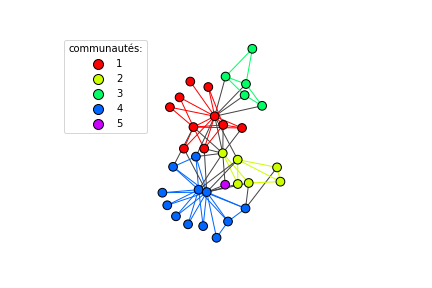
\includegraphics[scale=0.36]{images/G_zachary.png}%
			}%
			\hfill%
			\subfloat[communautés détectés pour le graphe généré aléatoirement]{%
				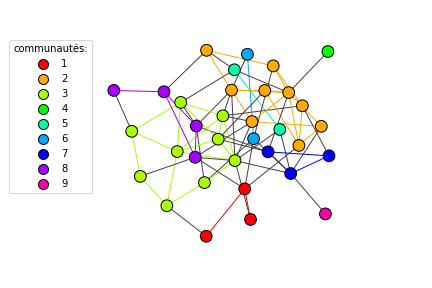
\includegraphics[scale=0.32]{images/random_network2.png}%
			}%
		\end{figure}
	\end{frame}
	

	


%	\begin{frame}{Cas des variables à "fortes séparations" }
%		\begin{figure}[htp] 
%			\centering
%			\subfloat[Boxplot des erreurs pour $\alpha_1$, $\alpha_2$ et $\alpha_3$]{%
%				\includegraphics[scale=0.18]{images/good_alpha.png}%
%			}%
%			\hfill%
%			\subfloat[Boxplot des erreurs pour $\mu_1$, $\mu_2$ et $\mu_3$]{%
%				\includegraphics[scale=0.18]{images/good_mu.png}%
%			}%
%		\end{figure}
%	\end{frame}

%	\begin{frame}{Cas des variables à "faibles séparations" }
%		\begin{figure}[htp] 
%			\centering
%			\subfloat[Boxplot des erreurs pour $\alpha_1$, $\alpha_2$ et $\alpha_3$]{%
%				\includegraphics[scale=0.18]{images/bad_alpha.png}%
%			}%
%			\hfill%
%			\subfloat[Boxplot des erreurs pour $\mu_1$, $\mu_2$ et $\mu_3$]{%
%				\includegraphics[scale=0.18]{images/bad_mu.png}%
%			}%
%		\end{figure}
%	\end{frame}
	

%	\begin{frame}{Préambule}
%		\begin{block}{Recueil des données}
%			\begin{figure}[H]
%				\centering
%				\includegraphics[scale=0.29]{tab_oiseaux.png}
%				\caption{Caractéristiques des nids; d'après [5]}
%			\end{figure}
%		\end{block}
%	\end{frame}	


	
	
	\section{Bibliographie}

	\begin{frame}
		\scriptsize
		\begin{enumerate}
		\item WikiStat. An introduction to network inference and mining,\textit{Article}\newline
		\url{http://www.nathalievialaneix.eu/doc/pdf/wikistat-network_compiled.pdf} \newline

		\item PNAS. Modularity and community structure in networks (2015),\textit{Article}\newline
		\url{https://www.pnas.org/doi/10.1073/pnas.0601602103\#abstract}

		\item Wikipédia (2022). Méthode de Louvain, \textit{Article}\newline
		\url{https://fr.wikipedia.org/wiki/Methode_de_Louvain} \newline

		\item igraph, \textit{Documentation}\newline
		\url{https://igraph.org/python/versions/latest/}\newline

		\item igraph, \textit{Documentation}\newline
		\url{https://igraph.org/python/versions/latest/tutorials/visualize_communities/visualize_communities.html}\newline

		\item igraph, \textit{Tutoriel}\newline
		\url{https://igraph.org/python/api/latest/igraph._igraph.GraphBase.html\#Erdos_Renyi}
		\end{enumerate}
	\end{frame}


\end{document}
